\documentclass[11pt, oneside]{article} 
\usepackage{geometry}
\geometry{letterpaper} 
\usepackage{graphicx}
	
\usepackage{amssymb}
\usepackage{amsmath}
\usepackage{parskip}
\usepackage{color}
\usepackage{hyperref}

\graphicspath{{/Users/telliott_admin/Dropbox/Tex/png/}}
% \begin{center} 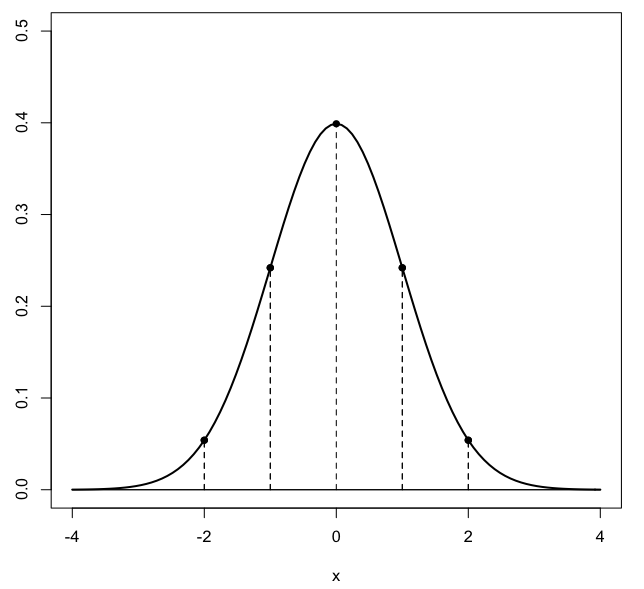
\includegraphics [scale=0.4] {gauss3.png} \end{center}

\title{Conservation of energy}
\date{}

\begin{document}
\maketitle
\Large

The law of conservation of energy is pretty simple in one dimension.  If kinetic energy ($T$) is 
\[ \frac{1}{2} mv^2 \]
then
\[ \frac{dK}{dt} = mv \frac{dv}{dt} = mva = Fv = F \frac{dx}{dt} \]
We just cancel the $dt$ and integrate:
\[ K_{2} - K_{1}  = \int_{x_1}^{x_2} F \ dx \]
\[ = U_1 - U_2 \]
where $U = - \int F \ dx$.  So
\[ U_1 + K_1 = U_2 + K_2 \]
 
To introduce the problem in two dimensions, I found a fun problem involving  the position vector and it uses dot notation for the time-derivative, so I put it here because we've done a lot of that in the chapters on Kepler.

The problem comes from Marsden and Tromba's \emph{Vector Calculus}.

First, we just state Newton's second law
\[ \mathbf{F} = m \mathbf{a} = m \mathbf{\ddot{r}} = m \frac{d^2}{dt^2} \ \mathbf{r} \]
and then make the statement that the force is minus the gradient of the gravitational potential V, which we've seen before
\[ \mathbf{F} = - \nabla V(\mathbf{r}) \]

The total energy in the system is the sum of the kinetic and potential energy:
\[ E = \frac{1}{2} m\ |\mathbf{\dot{r}}|^2 + V \]

And the problem given is to compute $d/dt$ of the energy.  According to the book, it's a "simple calculation."

Start with the first term, the kinetic energy.  Here is a trick to allow us to work with  $|\mathbf{\dot{r}}|^2$.  

Recall that
\[ \mathbf{\dot{r}} \cdot  \mathbf{\dot{r}}  = |\mathbf{\dot{r}}|^2 \]
and we looked at the time-derivative of the dot product of the velocity with itself earlier:
\[ \frac{d}{dt} \  \mathbf{\dot{r}} \cdot  \mathbf{\dot{r}} = 2\  \mathbf{\dot{r}} \cdot  \mathbf{\ddot{r}} \]

calling them "Feynman's dots".  This used the product rule. 

So then the time-derivative of the kinetic energy is
\[ \frac{d}{dt} \ \frac{1}{2} m\ |\mathbf{\dot{r}}|^2 = m\ \mathbf{\dot{r}} \cdot  \mathbf{\ddot{r}} \]
\[ = \mathbf{\dot{r}} \cdot \ [ \ m \ \mathbf{\ddot{r}} \ ] \]
\[ = \mathbf{\dot{r}} \cdot \ [ - \nabla V(\mathbf{r}) \  ] \]

To justify the last step, go back to the first two statements about the force, and equate them
\[ m \mathbf{a} = m \mathbf{\ddot{r}} = m \frac{d^2}{dt^2} \ \mathbf{r} =  - \nabla V(\mathbf{r}) \]

So now we need to evaluate this dot product.
\[ \mathbf{\dot{r}} \cdot \ [ - \nabla V(\mathbf{r}) \  ] \]

$V$ is a function of $x,y,z$ that yields a real number.  Its gradient is
\[ \nabla V = \ \langle \ \frac{\partial V}{\partial x},  \frac{\partial V}{\partial y},  \frac{\partial V}{\partial z} \ \rangle \]
while 
\[ \mathbf{\dot{r}} = \ \langle \frac{dx}{dt}, \frac{dy}{dt}, \frac{dz}{dt} \rangle \]
so the dot product is
\[  \nabla V \cdot  \mathbf{\dot{r}}  = \nabla V = \ \langle \ \frac{\partial V}{\partial x} \ \frac{dx}{dt},  \frac{\partial V}{\partial y} \ \frac{dy}{dt},  \frac{\partial V}{\partial z} \ \frac{dz}{dt} \ \rangle \]
\[ = \frac{d}{dt} V \]

We need to go back and pick up the minus sign we dropped from
\[ \mathbf{\dot{r}} \cdot \ [ - \nabla V(\mathbf{r}) \  ]  \ = - \frac{d}{dt} V \]

What was this?  We were calculating the time-derivative of the kinetic energy $T$.
\[ \frac{dT}{dt} = - \frac{dV}{dt} \]

And what was the problem?  It was to calculate the time-derivative of the total energy:
\[ E = T + V \]
\[ \frac{dE}{dt} =  \frac{dT}{dt} +  \frac{dV}{dt} =  -\frac{dV}{dt} +  \frac{dV}{dt} = 0 \]

And now we see it.  The total energy does not change with time.  This is the conservation law for energy.

\end{document}  